\section{Durchführung}
\label{sec:Durchführung}

\subsection{Versuchsaufbau}
\label{sec:Versuchsaufbau}
%\begin{figure}
%	\centering
%	\caption{Schematische Darstellung des Versuchsaufbaus \cite{anleitung}.}
%	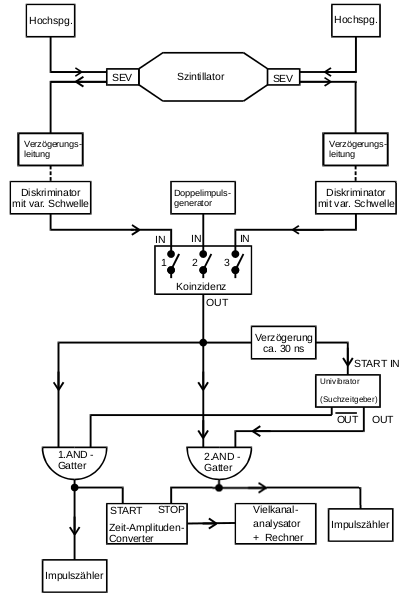
\includegraphics{Bilder/aufbau.png}
%	\label{fig:aufbau}
%\end{figure}
%
%\begin{figure}
%	\centering
%	\caption{Schematische Darstellung der Quelle zur Erzeugung radioaktiven Isotopen \cite{anleitung}.}
%	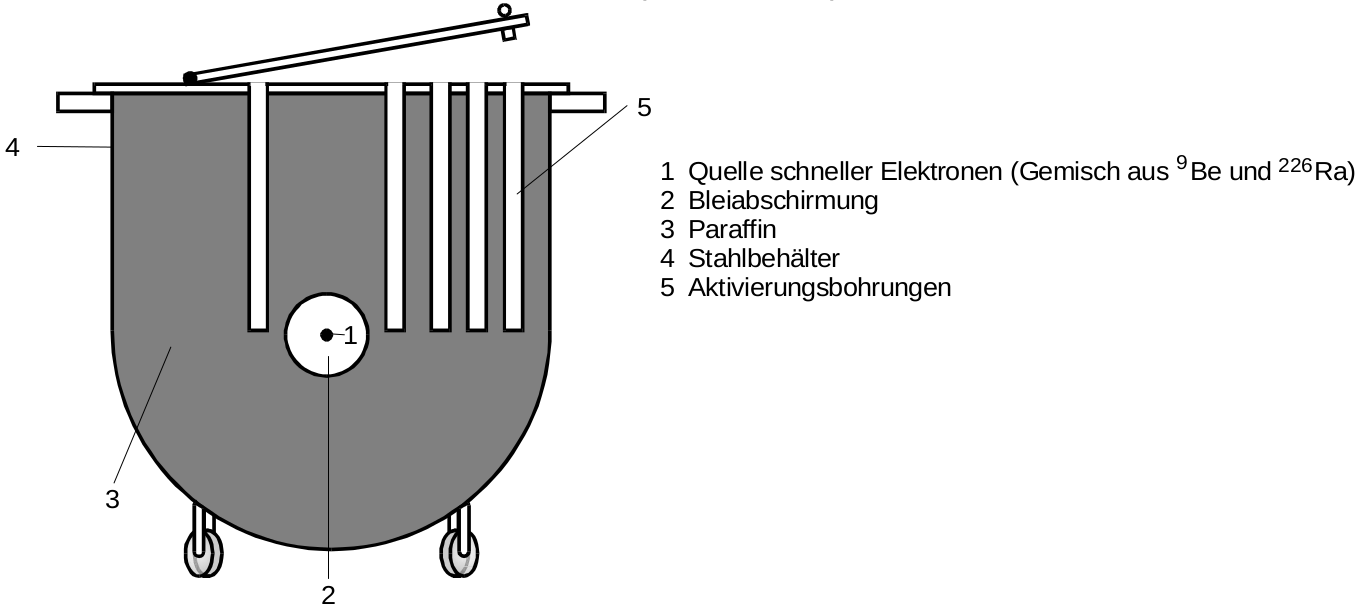
\includegraphics{content/toepfchen.png}
%	\label{fig:kochen}
%\end{figure}
%
Der Versuchsaufbau -- wie in Abbildung \ref{fig:aufbau} dargestellt -- besteht im Wesentlichen 
aus einem zerfallenden radioaktiven Isotop und einem Geiger-Müller-Zählrohr, welches die 
zerfallenden Kerne misst.
Das Geiger-Müller-Zählrohr ist entspricht einer mit Gas gefüllten Röhre. Trifft ein $\beta$-
oder $\gamma$- Teilchen auf ein Gasteilchen wird dieses ionisiert und kann aufgrund einer
anliegenden Spannung an der Röhre gemessen werden.
Dabei werden die gemessenen Zerfälle pro Messzeitintervall, welches am Zeitgeber einstellbar 
ist, an den Zählern 1 und 2 angezeigt. Nach jedem Messvorgang wird der Zähler umgeschaltet und 
der vorherige Wert auf dem aktuellen Zähler wird überschrieben. Der Versuchsaufbau ist mit
einer Blei-Abschirmung ausgestattet um die radioaktive Strahlung abzuschirmen.

Zur Erzeugung der radioaktiven Isotope wird das Objekt in Abbildung \ref{fig:kochen} verwendet.
Hierbei werden stabile Kerne mit niederenergetischen Neutronen beschossen. 
Da die Neutronen ihre Energie durch elastische Stöße an die Kerne übergeben und die maximale
Energie bei gleichen Massen der Stoßpartner erreicht wird, werden die Neutronen in einem 
Paraffinmantel gebremst, bis sie die optimale Energie besitzen.


\subsection{Versuchsbeschreibung}
\label{sec:Versuchsbeschreibung}
\subsubsection{Kalibration des Messaufbaus}
Zunächst wird der für die Rauschunterdrückung gedachte Teil des Versuchsaufbaus aufgebaut und mittels eines Oszillographen geprüft.
Nachdem die Hochspannung an den SEV eingeschaltet ist, werden die an den Ausgängen der SEV auftretenden Impulse unterschiedlicher Höhe zunächst vermessen.
Anschließend wird die Höhe der Diskriminatorimpulse gemessen. Zudem wird über ein Zählwerk die Zahl der pro Sekunde am Diskriminator auftretenden Impulse gemessen und die Diskriminatorschwellen an beiden Diskriminatoren so eingeregelt, dass etwa an beiden die gleiche Impulsrate mit etwa $20$ bis $40$ Impulsen pro Sekunde auftritt.
Da die Diskriminatoren nicht zur Filterung von Rauschsignalen dienen sollen, ist die Diskriminatorschwelle so zu wählen, dass eine möglichst hohe Impulsrate auftritt.
Beide Signale werden anschließend auf die Koinzidenzschaltung aufgegeben und am Ausgang der Koinzidenz wird die Zählrate  in Abhängigkeit der Verzögerung gemessen. Es bildet sich ein Maximumsplateau aus, innerhalb dessen die Verzögerungszeit zu wählen ist, welche bei der späteren Lebensdauermessung verwendet wird.
Aus der Messung lässt sich zudem die Koinzidenzzeit $\Delta t_{\mathrm{K}}$ der Koinzidenz bestimmen.
Geprüft wird außerdem, ob die Zählrate hinter der Koinzidenz kleiner ist als vor ihr. Ist dies nicht der Fall, wäre sie wirkungslos. Die Diskriminatorschwellen müssen dann entsprechend etwas abgesenkt werden.
Für die weitere Kalibrierung der Schaltung wird ein Doppelimpulsgenerator an die Koinzidenzschaltung gelegt.
Die Zeit zwischen zwei durch den Doppelimpulsgenerator erzeugten Impulsen lässt sich dabei mit einer Genauigkeit von $\SI{0.1}{\micro\second}$ einstellen.
Die monostabile Kippstufe wird nun wie in Abbildung \ref{fig:aufbau} gezeigt, in die Schaltung eingebaut und an ihrem Ausgängen ihre Funktionalität geprüft. Die Suchzeit des Univibrators wird auf $T_{\mathrm{S}}=\SI{20}{\micro\second}$ eingestellt.
Nachdem nun ebenfalls die AND-Gatter eingebaut werden, ist an deren Ausgängen zu prüfen, dass sich diese um genau den Zeitabstand unterscheiden, welcher am Doppelimpulsgenerator eingestellt wurde.
Zudem wird geprüft, dass die Signalhöhe am Ausgang des TAC proportional zum eingestellten Impulsabstand ist.
Anschließend wird noch durch Variation der Impulsabstände geprüft, welcher Kanal am Mehrkanalanalysator welchem Zeitabstand entspricht. Über eine Zuordnung der Impulsabstände zu den Kanälen kann schließlich der Vielkanalanalysator kalibriert werden.

\subsubsection{Ablauf der Messung}
Die Messung wird begonnen, indem sowohl das Zählwerk als auch der Vielkanalanalysator gestartet werden.
Nach einer Messung von etwa $26$ Stunden, wird die Messung über das Stoppen des Zählwerks und des Vielkanalanalysators beendet.
Aufgezeichnet wird die Anzahl der tatsächlichen Myonenzerfälle, die Anzahl der aufgetretenen Eintrittsimpulse, die Ergebnisse des Vielkanalanalysators sowie die Messzeit, welche sich am Vielkanalanalysator ablesen lässt.
